\cotefile{19}
\scanpage{19}
3) Une suite

\[
0\to A'\unsure{-|\to} A\to A''-0 \tag*{(1)}
\]
dans $\mathcal C$ est dite $S$-exacte si la suite
\[
0-S(A')-S(A)\to S(A'')-0 \tag*{(1 bis)}
\]
\deleted{est exacte et} \inserted{est ``exacte et} \uline{se scinde}''.

Un objet $M\in\mathcal C$ est dit $S$-injectif, si pour toute suite $S$-exacte (1), la suite
\[
0-\mathrm{Hom}(A'',M)-\mathrm{Hom}(A,M)\longrightarrow\mathrm{Hom}(A',M)-0 \tag*{(2)}
\]
est exacte.

\uline{Exemples} (i) $M=T(X)$, car alors la suite (2) \unsure{s'écrira|s'écrit}
\[
0\to\mathrm{Hom}(S(A''),X)\to\mathrm{Hom}(S(A),X)-\mathrm{Hom}(S(A'),X)-0. \tag*{(2 bis)}
\]

[D'ailleurs, si (1) est telle que pour \deleted{tout} objet $S$-injectif $M$, \unsure{ou|on} \deleted{\unsure{particulièrement}} \inserted{\unsure{même}} seulement pour \unsure{tt} objet de la forme $M=\unsure{T|F|S}(X)$, \deleted{\unsure{avec} $X\in\mathcal C'$, (et même \unsure{seult} $X=S(A')$),} la suite (2) est exacte, alors (1) est $S$-exacte, car \deleted{(1 bis)} (2 bis) sera exacte pour \deleted{\unsure{tout} $X$ \illegible{2} pour $X=S(A')$,} \inserted{tt $X$, donc (1 bis) exacte}]

\deleted{\unsure{en} fait, il suffit de \unsure{prendre|fixer} $X$ \unsure{pour} \illegible{3} \unsure{Homomorphisme identique} de $S(A')$, et si $S$ est un foncteur exact à droite, alors il suffit pour $A'\to A-A''-0$ soit exacte, et que la suite}

(ii) Supposons $S$ \uline{exact} \inserted{à droite} \deleted{et ``fidèle'' en ce sens que} $S(u)=0\Longrightarrow u=0$. Soit $A\in\mathcal C$, je dis que la suite

\[
\deleted{\unsure{\Sigma}}\,\Sigma(A):\quad 0-A\to TS(A)\longrightarrowZ(A)-0 \tag*{(3)}
\]

(où $Z(X)=\mathrm{Coker}(X-TS(X))$) est $\unsure{S|\Sigma}$-exacte. En effet, \deleted{elle} se transforme par $S$

% archive sheet number: 18
\scanpage{20}
en
\[
0\unsure{-|\to}S(A)-STS(A)-S\unsure{Z|\zeta}(X)\longrightarrow0
\]

elle est exacte en $STS(A)$ et $SZ(X)$ puisque $S$ est exact à droite, et exacte à gauche et \unsure{splittée} car on a \unsure{explicitmt|explicitement|explicite} un inverse à \deleted{droite} gauche de $S(A)\to S(TS)(A)=(ST)S(A)$.

[ Soit $M\in\mathcal C$ \unsure{telle|tel} que pour \deleted{\unsure{tt|toute}} suite \deleted{de la} $S$-exacte de la forme $\Sigma(A)$, la suite transformée $\mathrm{Hom}(\Sigma(A),M))$ soit exacte :
\[
0-\mathrm{Hom}(Z(A),M)-\mathrm{Hom}(TS(A),M)-\mathrm{Hom}(A,M)\to0
\]

Alors $M$ est $S$-injectif. En effet, on fera $M=A$, et on trouve que $A-TS(A)$ identifie $A$ à un \uline{facteur direct} de $TS(A)=T(X)$ $(X=S(A))$. Or $T(X)$ est $S$-injectif en vertu de (i), donc \deleted{tout} facteur direct l'est, donc $A$ l'est. On voit en \unsure{$=$} temps que $M$ $S$-injectif $\Longleftrightarrow$ $M\to TS(M)$ est un isomorphisme sur un facteur direct (cf les faiblement injectifs de Cartan Eilenberg).

\uline{Remarque} Supposons \deleted{que le foncteur $S$ soit exact} \inserted{le foncteur $S$ exact \deleted{à droite}} \deleted{et} que $S(u)=0$ implique $u=0$, \inserted{i.e. $\varphi$ est \uline{injectif}.} Alors une suite $S$-exacte \inserted{\unsure{(1)|($\Sigma$)}} est exacte. En effet, \deleted{pour \unsure{tout} $A\in\mathcal C$} \deleted{$S$\unsure{pour} \illegible{1}} si $\Sigma:P\xrightarrow{u}Q\overset{v}{-}R$ et $S(v)S(u)=0$, \deleted{\unsure{alors|donc}} \inserted{i.e.} $S(vu)=0$, alors

% archive sheet number: 19
\scanpage{21}
\deleted{\unsure{Le} \illegible{2} \unsure{donne}} \deleted{\inserted{Considérons le diagramme}}

\diagram{\begin{tikzcd}[ampersand replacement=\&,column sep=small]
\deleted{0}\arrow[r,dash] \& \deleted{\mathrm{Hom}(B,A')}\arrow[r,dash]\arrow[d] \& \deleted{\mathrm{Hom}(B,A)}\arrow[r,dash]\arrow[d] \& \deleted{\mathrm{Hom}(B,A'')}\arrow[r] \& \deleted{0}\\
\deleted{0}\arrow[r,dash] \& \deleted{\mathrm{Hom}(SB,SA')}\arrow[r] \& \deleted{\mathrm{Hom}(SB,SA)}\arrow[r,dash] \& \deleted{\mathrm{Hom}(\unsure{SB|B},SA'')}\arrow[r] \& \deleted{0}
\end{tikzcd}}

\deleted{alors les deux flèches verticales et la \unsure{deuxième|dernière} horizontale sont injectives, donc aussi la première horizontale, donc $B'\unsure{-|\to}B$ est injectif. En prenant $\mathrm{Hom}(S,B)$, on voit de $=$ que $B-B''$ est surjectif, d'autre part $S$ étant injectif, le composé $B'\to B\to B''$ \deleted{\unsure{est}} est nul.}

$vu=0$, et on aura $S(\mathrm{Ker}\,v/\mathrm{Im}\,u)=\mathrm{Ker}\,S(v)/\mathrm{Im}(Su)$ et le \deleted{\unsure{de|des}} premier \unsure{mb} est nul si et seulement si $\mathrm{Ker}\,v/\mathrm{Im}\,u$ l'est, on voit que $\Sigma$ est une suite exacte si et seulement si $S$ l'est.

\figure{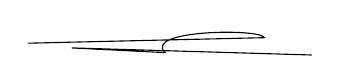
\begin{tikzpicture}[x=1cm,y=1cm]\draw (0,.10)--(3,.17).. controls (2.95,.29) and (1.45,.27) .. (1.74,-.02)--(.55,.04)--(3.6,-.05);\end{tikzpicture}}

Nous avons maintenant ce qu'il faut [catégorie de ``suites exactes'' $\Longleftrightarrow$ catégorie d'``injectifs''] pour faire une théorie ``relative'' des foncteurs dérivés $\mathcal C\to\mathcal D$, où $\mathcal D$ est une véritable catégorie \uline{abélienne}. De plus, \inserted{une} \deleted{\unsure{l'}}itération des foncteurs $TS=C^0$ :

\[
C^1(A)=C^0(A)/\mathrm{Im}\,A\qquad C^i(A)=C^0(C^{i-1}(A)/\mathrm{Im}(C^{\deleted{\unsure{i}}i-2}(A)))\quad\text{si }i\geq2 .
\]

donne une résolution \inserted{$S$-injective} \uline{canonique} (fonctorielle) de $A\in\mathcal C$

% archive sheet number: 20
\scanpage{22}
\deleted{\illegible{1} $A\in\mathcal C$. La construction}

Dans le cas où $\mathcal C$ est une catégorie \uline{abélienne} ayant déjà suffisamment d'injectifs, la question se pose de savoir quand les foncteurs dérivés droits \inserted{usuels} d'un foncteur $\Gamma:\mathcal C\unsure{-|\to}\mathcal D$ coïncident avec les foncteurs dérivés usuels. \deleted{Voici des} \inserted{Voici des} conditions suffisantes raisonnables. On veut tout au moins que $R_S^*\Gamma$ soit un foncteur cohomologique,

\deleted{Supposons que $\varphi$ soit injectif, i.e. $A\to TS(A)$ injectif pour tout $A\in\mathcal C$. \unsure{Supposons} $\Gamma$ exact \unsure{à gauche}. \illegible{2} $S$ et $T$ exacts, donc $TS$ exact, donc que la résolution canonique $C(A)$\unsure{?} La $S$-résolution canonique de $A$ est une résolution au sens usuel, d'où résulte que $R^0_S\Gamma=\Gamma=R^0\Gamma$. Il \unsure{reste|vaut} donc à prouver l'effaçabilité des $R_S^p\Gamma$}

i.e. l'opérateur cobord $\partial$ est défini pour \uline{\unsure{ttes}} les suites exactes en $A'-A-A''-0$ (et ``non seulement'' les suites $S$-exactes). C'est \unsure{le|le le|donc le} cas si $\Gamma(C^*(A))$ est un foncteur exact en $A$, pour ceci nous supposons.

% margin note written sideways
\margin{Ces conditions d'ailleurs suffisent, car \deleted{\unsure{alors}} $(R_S^*\Gamma)$ sera aussi \unsure{coeffaçable|effaçable}, car il s'annule \deleted{\unsure{évidemment}} sur les objets de la forme $T(X)$, qui sont ``assez nombreux'' grâce à (i). \deleted{soit un foncteur \uline{exact} par r. à $A$.}}

(i) $A\to C^0(A)$ injectif

(ii) $S$ et $T$ [donc $C^0$, donc \inserted{aussi} $C^*$ \inserted{compte tenu de (i)}] foncteurs exacts

(iii) Si $0\to A'-A-A''-0$ est une suite exacte de $\mathcal C$, alors la suite $0-\Gamma C^0(A')\to\Gamma C^0(A)-\Gamma C^0(A'')\inserted{-0}$ est exacte [Il suffit que le foncteur \uuline{$\Gamma T$ soit exact}]

\deleted{Enfin, pour} \inserted{Alors} $R^*_S\Gamma$ est bien un foncteur cohomologique. Pour qu'en degré $0$, il coïncide avec $R^0\Gamma$, on va supposer que

\unsure{(iv)} \deleted{\unsure{les} \illegible{1} $A\to C^0(A)$ injectifs} $\Gamma$ exact à gauche.

% archive sheet number: 21
\scanpage{23}
Exemples : (i) si \raisebox{.6ex}{(8)} $\boxed{M=T(N)}$ car alors la suite (6) s'identifie à \deleted{\unsure{la}}
\[
0\to\mathrm{Hom}(\widetilde A'',\widetilde N)\unsure{-|\to}\mathrm{Hom}(\widetilde A,\widetilde N)-\mathrm{Hom}(\widetilde A',\widetilde N)\to0
\]

D'ailleurs, si (6) est telle que, pour tt $M=T(N)$, la suite (7) est exacte, alors (6) est $\sim$-exacte.

\deleted{Si $M$ est $\sim$-injectif, \unsure{alors la suite} $0-M\xrightarrow{i_M}T(M)\xrightarrow{\alpha}M'-0$, où $M'=\mathrm{Coker}\,i_M$, \illegible{1} \unsure{exacte}}

\inserted{\fbox{Supposons le foncteur $\sim$ \uline{exact} et ``fidèle''}}

% slanted
\margin{\unsure{p} alors les suites $\sim$-exactes sont \uline{exactes} (car pour qu'une suite $K$ \inserted{\unsure{comme on aura} $\widetilde{\mathrm H(K)}=\mathrm H(\widetilde K)$} \deleted{\illegible{2}} de $\mathcal C$ soit exacte, il f. et s. que $\widetilde K$ le soit)}

(ii) Soit \deleted{$\unsure{A}\in\mathcal C$} \inserted{$X\in\mathcal C$}, la suite \deleted{$0-A\xrightarrow{i_A}T(A)-A'-0$}
\[
\boxed{S_X:\quad0-X\overset{i_X}{-}T(X)-X^*-0}\tag*{(9)}
\]
\deleted{$\unsure{A'}$} $\unsure{X'|X^*}=\mathrm{Coker}\,i_X$, est $\sim$-exacte. En effet,

elle est transformée en \deleted{\unsure{deux}} suite exacte
\[
\deleted{\unsure{S(X)|S(S_X)}:}\quad 0-\widetilde X\xrightarrow{\widetilde i_X}T(\widetilde X)\to\widetilde {X^*}-0
\]
, qui \deleted{\unsure{splitte|scindée}} \inserted{se scinde} (canoniquement) en vertu de (4).

Supposons alors que \inserted{$M\in\mathcal C$ soit tel} que \uline{tte} \deleted{\unsure{telle|toute}} suite exacte de cette forme, la suite (7) soit exacte, \inserted{je dis que $M$ est $\sim$-injectif.} Cela sera vrai en particulier si \deleted{\unsure{$A$}} $X=M$ pour $0-M-T(M)-M^*-0$, donc $M$ est facteur direct de $T(M)$. Ce dernier étant $\sim$-injectif, il en est \deleted{\unsure{donc}} de $=$ de $M$.

Ceci montre aussi : les objets injectifs sont exactement les facteurs directs des objets $T(M)$.
\deleted{\unsure{les} \illegible{2} \unsure{caractérisés} \illegible{2} facteurs directs des}

% paper watermark: ARGENTINE TYPEWRITER (repeating, mirrored and partly cropped)
% archive sheet number: 22
\scanpage{24}
\deleted{objets $S$ pour lesquels il existe une suite $\sim$-exacte de \deleted{\unsure{suites}} \inserted{complexes} \deleted{suites du type $S(X)$.} $0\to S\to S(X)\to S^*-0$. [pour le voir, on écrit, si $0\unsure{-|\to}A'-A-A''-0$ est $\sim$-exacte,}

% slanted
\margin{Dorénavant, $\sim$ est exact et ``fidèle''}

\diagram{\begin{tikzcd}[ampersand replacement=\&,column sep=small]
\deleted{0}\arrow[r,dash] \& \deleted{A'}\arrow[r,dash,"\deleted{u}"]\arrow[d,"\deleted{\unsure{i_{A'}u|i_{A'} }}"] \& \deleted{A}\arrow[r,dash,"\deleted{v}"]\arrow[d,"\deleted{i_A}"] \& \deleted{A''}\arrow[r,dash]\arrow[d] \& \deleted{0}\\
\deleted{0}\arrow[r,dash] \& \deleted{T(\unsure{A|A'})}\arrow[r,"\deleted{\unsure{i_A|u}}"'] \& \deleted{\unsure{T(T(A))|TT(A)}}\arrow[r,dash] \& \deleted{\unsure{T(A)^*}}\arrow[r] \& \deleted{0}
\end{tikzcd}}

\figure{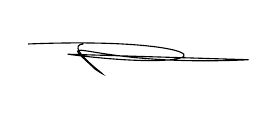
\begin{tikzpicture}[x=1cm,y=1cm]\draw (0,.2).. controls (2.5,.3) and (2.6,-.2) .. (.5,.07)--(2.8,0).. controls (.7,-.1) and (.3,.4) .. (.85,-.12).. controls (1.2,-.35) and (.4,.18) .. (.7,.2);\end{tikzpicture}}

Une $S$-résolution d'un $A\in\mathcal C$ est une résolution \deleted{\illegible{1}} $X$ de $A$, \uline{munie} d'un opérateur d'homotopie \deleted{\illegible{1}} \unsure{$s$} dans le complexe augmenté $0-\unsure{\widetilde A|\bar A}-\widetilde X^0-\widetilde X^1-\widetilde X^{\unsure{2|3}}-\ldots$ i.e. de projections \inserted{splittantes} dans les suites exactes

\[
0-Z^i(X^*)-X^i\to Z^{i+1}(X^*)-0\qquad (i\geq0)
\]

\deleted{\uline{Proposition} \unsure{Soit} $X$ \unsure{une résolution|projectifs}}
\deleted{Un \deleted{application} \inserted{morphisme} \deleted{$\unsure{f}:$ \illegible{1}} $\unsure{\eta|y}:X\to Y$ de $\mathcal C$ est dit \deleted{\unsure{spécial} \unsure{spéciale}} \inserted{effaçant} si \deleted{$\widetilde X-\widetilde Y$ est} pour tout $A\in\mathcal C$, l'image de $\mathrm{Hom}(\widetilde A,\widetilde X)$ dans $\mathrm{Hom}(\widetilde A,\widetilde Y)$ par $u\to\widetilde\eta\,\widetilde u$ est contenue dans l'image de $\mathrm{Hom}(A,Y)$, i.e. si on a un diagramme commutatif}

\diagram{\begin{tikzcd}[ampersand replacement=\&,column sep=large]
\deleted{\mathrm{Hom}(\widetilde A,\widetilde X)}\arrow[r,"\deleted{\unsure{u}\,-\,\widetilde\eta\widetilde u}"]\arrow[dr] \& \deleted{\mathrm{Hom}(\widetilde A,\widetilde Y)}\\
\deleted{\mathrm{Hom}(A,T(X))}\arrow[u,"\deleted{\unsure{\sim}}"'] \& \deleted{\mathrm{Hom}(A,Y)}\arrow[u,"\deleted{\sim}"]
\end{tikzcd}}

% paper watermark: ARGENTINE TYPEWRITER (vertical, partly cropped)
% archive sheet number: 23
\scanpage{25}
\diagram{\begin{tikzcd}[ampersand replacement=\&,column sep=large]
\deleted{\mathrm{Hom}(\widetilde A,\widetilde X)}\arrow[r,"\deleted{u-\widetilde{\unsure{g|\eta}}\widetilde u}"]\arrow[ddr,"\deleted{\rho_A}"] \& \deleted{\mathrm{Hom}(\widetilde A,\widetilde Y)}\\
\deleted{\mathrm{Hom}(A,T(X))}\arrow[u,"\deleted{\sim}"]\arrow[r,"\deleted{u\to T(g)u}"] \& \deleted{\mathrm{Hom}(A,T(Y))}\arrow[u,"\deleted{\sim}"]\\
\&\deleted{\mathrm{Hom}(A,Y)}\arrow[u]
\end{tikzcd}}

\deleted{où $\beta_A$ est évidemment unique. Il revient au $=$ de dire que l'application \deleted{\illegible{1}} $T(g):T(X)\unsure{-|\to}T(Y)$ se factorise en $T(X)\longrightarrow Y\xrightarrow{i_Y}T(Y)$. \unsure{Disons|Disons nous|On voit}, que $g$ \uline{efface} le foncteur $T(X)/i_X(X)$ \deleted{\unsure{On convient que|Démonstration, que}}}

\deleted{\uline{Exemple} Si $g$ est un morphisme \unsure{spécial|quelconque} il en est de $=$ de $\lambda g$ quel que soit $\lambda\in\mathrm{Hom}(Y,\unsure{Z})$.}

\deleted{Un morphisme \deleted{\illegible{1}} \deleted{\unsure{$g$}} $i_M:M-T(M)$ est tjrs effaçant}

On appelle $t$-\deleted{résolution d'un} \inserted{complexe droit sur un} objet $A\in\mathcal C$ un complexe \inserted{droit} $X$ sur $A$, $A\to X$, muni de morphismes $t:T(A)-X^0$, $T(X^i)-X^{i+1}$ $(i>0)$ rendant commutatifs les diagrammes

\diagram{\begin{tikzcd}[ampersand replacement=\&]
A\arrow[r,"i_A"]\arrow[dr,"\varepsilon"'] \& T(A)\arrow[d,"t"]\\
\&X^0
\end{tikzcd}}

\diagram{\begin{tikzcd}[ampersand replacement=\&]
X^i\arrow[r,"i_{X^i}"]\arrow[dr,"d^i"'] \& T(X^i)\arrow[d,"t"]\\
\&X^{i+1}
\end{tikzcd}}

\deleted{Soit alors $t$} Soit donc $\unsure{A|A'}\to X$ une $s$-résolution \deleted{de} $A$, $B\to Y$ un $t$-complexe droit sur $B$, et $u:A\to B$

% paper watermark: ARGENTINE TYPEWRITER (vertical, ends cropped)
% archive sheet number: 24
\scanpage{26}
un morphisme, on va prolonger $u$ \deleted{de} façon \uline{canonique} en un \unsure{hom.} $\bar u$ de $X$ dans $Y$ compatible avec les augmentations. Si on a déjà défini $\bar u^n:X^n\unsure{-|\to}Y^n$ \deleted{\unsure{et}} pour un $n$ $(n\geq-1)$, montrons comment continuer : \unsure{on a} $s^{n+1}\in\mathrm{Hom}(\unsure{\overline{X^{n+1}}|\widetilde{X^{n+1}}},\overline{X^n})$,

\diagram{\begin{tikzcd}[ampersand replacement=\&]
X^n\arrow[r,"d^n"]\arrow[d,"\bar u^n"']\& X^{n+1}\\
Y^n\arrow[r,dash,"d^n"]\&Y^{n+1}\\
\unsure{\vert|1}\&
\end{tikzcd}}

\deleted{il définit} \inserted{soit} $s'^{n+1}\simeq\mathrm{Hom}(\deleted{\unsure{\widetilde X}}X^{n+1},T(X^n))$ définit un \deleted{\unsure{hom}} morphisme $\deleted{\unsure{t}}T(\bar u^n)\circ s'^{n+1}:X^{n+1}-T(Y^n)$, d'où, \deleted{\illegible{1}} \inserted{composant avec le} morphisme $t^n:T(Y^n)-Y^{n+1}$, un morphisme \deleted{$\unsure{X^i}$} $t^nT(\bar u^n)s'^{n+1}:X^{n+1}\to Y^{n+1}$, posons

\[
\bar u^{n+1}=t^nT(\bar u^n)s'^{n+1}
\]

\deleted{On a $\bar u^{n+1}d^n=t^nT(\bar u^n)s'^{n+1}d^n=-t^nT(\bar u^n)d$}

On vérifie que ça marche \unsure{\ldots}.

\uline{Résolution canonique} $C^*(A)$, définie par
\[
C^{n+1}(A)=T(C^n(A)/\mathrm{Im}\,\widehat C^{n-1}(A))\quad (\deleted{\unsure{en|\text{avec}}}\ \text{posant }\widehat C^{-1}(A)=A)
\]

\deleted{$\unsure{C^*(A)|C^\bullet}$} C'est à la fois une $s$ et une $t$-résolution, c'est un foncteur en $A$. L'hom fonctoriel $C^*(A)-C^*(B)$ associé à un hom $A-B$ est en fait celui défini grâce à la $s$-structure de $C^*(A)$ et la $t$-structure de $C^*(B)$.

% paper watermark: ARGENTINE TYPEWRITER (mirrored, vertical)
% archive sheet number: 25
\scanpage{27}
\deleted{Structures multiplicatives}

\uline{Exemples} 1) Soient $U$ un anneau, $V$ un sous-anneau, considérons le foncteur
\[
\mathcal C=\mathcal C^U\to\widetilde{\mathcal C}=\mathcal C^V\qquad\text{restriction des scalaires}
\]

C'est un foncteur \uline{exact}, et les applications $\mathrm{Hom}(A,B)\longrightarrow\mathrm{Hom}(\bar A,\bar B)$ sont injectives. De plus, on a
\[
\begin{aligned}
\mathrm{Hom}_{\unsure{V}}(\widetilde A,\widetilde B)&=\mathrm{Hom}_V(A,B)\xrightarrow{\sim}\deleted{\mathrm{Hom}_U(\unsure{A|U\otimes_V A},\unsure{B})}\\
&\inserted{\mathrm{Hom}_U(A,\underbrace{\mathrm{Hom}_V(U,B)})}
\end{aligned}
\]

\margin{$U$-module gauche (grâce à \unsure{$U$}) \deleted{\unsure{la multiplication}} \unsure{via la} \deleted{\unsure{action}} \unsure{multiplication|mult\textsuperscript{on}} de $V$ sur $U$}

cet \deleted{hom.} \inserted{isom} est donné grâce \deleted{au} \unsure{le|à|de} $V$-hom naturel \deleted{(Obtenu en} \deleted{\unsure{faisant} \illegible{1} $B$ \unsure{$\mathrm{Hom}_U(A,B)$|$\mathrm{Hom}_U(U,B)$} $B\to\mathrm{Hom}_V(U,B)$}
\[
e_B:\mathrm{Hom}_V(U,B)\longrightarrow B
\]

défini par \deleted{\unsure{$f$}} $e_B(f)=f(1)$. L'hom. (sur $U$) naturel correspondant
\[
i_B:B\unsure{-|\to}\deleted{\mathrm{Hom}_{\unsure{V}}(U,B)}\mathrm{Hom}_V(U,B)
\]
est celui qui résulte de $B\xrightarrow{\sim}\mathrm{Hom}_U(U,B)\to\mathrm{Hom}_V(U,B)$.

Les suites \deleted{\unsure{$S$}} $\sim$-exactes sont celles qui splittent sur $V$. Les $U$-modules $\sim$-injectifs sont les facteurs directs de modules $\mathrm{Hom}_V(U,B)$.

% paper watermark: ARGENTINE TYPEWRITER (vertical, partly cropped)
% archive sheet number: 26
\scanpage{28}
2) On a aussi $\mathrm{Hom}_V(A,B)=\mathrm{Hom}_U(U\otimes_V A,B)$

Ce qui nous ramène à la \inserted{situation} \uline{duale} de \uline{celle} \deleted{que} envisagée dans les généralités précédentes. \deleted{\unsure{Mais}}

[On voit donc que les objets \deleted{\unsure{$S$}} $\sim$-projectifs sont les facteurs directs d'objets $U\otimes_V A$.]

Ici les hom. canoniques \deleted{\unsure{sont}}

\[
\begin{aligned}
&\deleted{U\otimes_V A\to A}\\
e_A^*:\quad & A\longrightarrow U\otimes_V A \qquad (V\text{-linéaire, donné par }a\unsure{-|\to}1\otimes a)
\end{aligned}
\]

\[
i_A^{+}:\quad U\otimes_V A-A \qquad (U\text{-linéaire surjectif par }u\otimes_V a-\unsure{ua|au})
\]

3) Soit $\mathcal C$ la catégorie des faisceaux de $\underline O$-modules sur $X$, et $\widetilde{\mathcal C}$ la catégorie produit $\prod_{x\in X}\mathcal C^{\underline O_x}$

On a la \unsure{solution|situation} du pb. universel grâce au foncteur de Godement $F-C^0(F)$. \quad ---

% paper watermark: ARGENTINE TYPEWRITER (vertical; reverse of sheet shows through)
% archive sheet number: 27
\scanpage{29}
\uline{\unsure{Remords|Renvois|Remarques}}

11 p

SGA 4 $\underline{\overline{\mathrm{IX}}}$

\figure{\begin{tikzpicture}[x=1cm,y=1cm]\draw (0,.3)--(.1,0);\end{tikzpicture}}

\unsure{7|J}

% archive sheet number: 28
\scanpage{31}
\deleted{\unsure{VIII|IX|VII}} \uline{IX}

1. Suite des faisceaux de torsion

2. Faisceaux loc. constants.

3. Faisceaux constructibles

\uline{\unsure{Préciser|Précise} nos conventions}. Qu'est-ce que veut dire loc. ct. à fibres finies sur $X^{\mathrm{cons}}$. Le reste du n° 2 donne les propriétés de commutation de la notion

\textcircled{a} \uline{Conditions équivalentes}\,: (i) L'image inverse sur $X^{\unsure{\mathrm{ens}|\mathrm{cons}|\mathrm{red}}}$ est loc. ct à fibres finies

(ii) $\exists\ f:X'\unsure{-|\to}X$ loc. de présentation finie surjectif, avec $f^*(F)$ loc. ct à fibres finies

(iii) \deleted{Si} Si $X$ qu. cp et qu. sép) $\exists$ partition de $X$ en $X_i$ loc. fermés constructibles, en nb fini, t.q. $F|X_i$ loc. ct. à fibres finies.

(iv) \inserted{(Si $X$ qu. cp et qu. sép)} $F$ est le conoyau d'une double flèche
\[
\deleted{\unsure{F_1}} F_{\unsure{1|2}}\rightrightarrows F_0,
\]
où $F_0$ et $F_{1}$ sont des faisceaux repr. par des schémas étales de prés. finie sur $X$

(v) \inserted{($X$ qu. cp et qu. sép)} $F$ est \deleted{du type} \inserted{coker d'} \unsure{constructiblement|constructibles} de type fini, et tt \unsure{hom} d'un faisceau \deleted{\unsure{repr}} $G$ dans $F$, avec $G$ repr. par pr. étale de prés finie sur $X$, \deleted{\unsure{le}} la \unsure{rel.} équiv. est constr.

(vi) \inserted{($X$ qu. cp et qu. sép\,; Gr. abéliens \deleted{\unsure{$F$}} et \unsure{cat})} $F$ admet une filtration par des $i_!(G)$, $i:Y-X$ imm. \inserted{constr.} \deleted{qu. cp \unsure{et}}, $G$ \deleted{\unsure{repr est}} sur $Y$

(vii) ($X$ qu. cp et qu. sép.\,, Gr abéliens, $A$ et \unsure{autres})\,:\enspace $F$ admet une \deleted{\unsure{prés}} résolution \inserted{à deux crans} par des \unsure{$p_* (\mathbb Z_{X'})$|$p_*(G_{X'})$}, $X'$ fini de prés finie sur $X$, $G$ ct. \unsure{constr.}

% slanted
\margin{Pour \unsure{dévisser en|l'énoncé} \unsure{catégorie|algèbre} les faisceaux de torsion}

\inserted{Si $A=\mathbb Z$, faisceaux de l-torsion, $X$ qu. cp et qu. sép)} (viii) \deleted{\unsure{Si $F$ est constructible et $X$ localement} \illegible{3} \unsure{volumes} \illegible{2}} $F$ se dévisse par \deleted{\unsure{faisceaux}} \inserted{suite de cinq} \unsure{termes} en faisceaux \inserted{finis} dont des quotients facteurs directs d'un faisceau lié, \unsure{admettant} une suite de composition par des faisceaux de la forme $p_*(i_!(\mathbb Z/\ell\mathbb Z)_U)$, où $p:X'-X$ mo. fini surj., fini \inserted{et de} \deleted{\unsure{prés}} prés., $U$ ouvert \unsure{dense} de $X'$, $i:U-X'$ l'inclusion

On peut \unsure{couper|songer} avec des complexes de $\mathcal A$-Modules et la \unsure{$K$|$A$}-constructibilité

Au vu de ces rédactions, il sera bon de convenir pour la \unsure{$0$|$a$|$\mathbb Q$}- et la $1$-constructibilité.

\textcircled{b} \uline{Déf} Constructibles de type fini, resp. constr. de prés finie = constructibles

\deleted{et \unsure{constr. égaux}}

\uline{Cor} \textcircled{c} Stabilité par $\underset{\longrightarrow}{\lim}$ et $\underset{\longleftarrow}{\lim}$ finies (dans le cas abélien, il faut \deleted{et \unsure{eff}} que $A$ \unsure{noeth. resp.|soit un corps.} $\mathcal A$ soit \unsure{ann. cohérent}), pr \uline{facteurs} \uline{directs}.

\uline{Cor} \textcircled{d} Caractère épais (\unsure{Grs comm.|Grs non-comm.|cas noethérien})

\uline{Cor} \textcircled{e} Stabilité par image inverse. par image directe par morph fini de prés. finie \deleted{par image directe par} \deleted{\unsure{implication finie de prés. finie}}

% archive sheet number: 30
\scanpage{32}
\deleted{\uline{Pureté}}

\deleted{\uline{Proposition} Soit $X$ un préschéma loc. noeth. \uline{régulier}.}

\deleted{Conditions équivalentes}

\deleted{(i) Pour tt sous-préschéma régulier $Y$ de $X$, et tout sous-préschéma régulier fermé $Z$ de $Y$, partout de codim $d$, on a}
\[
\deleted{\left\{\begin{aligned}
\underline H^{\unsure{i|i'}}_Z(A_Y)&=0 &&\text{pour } i\ne2d\\
\deleted{\underline H^{2d}_Z(A_Y)}&\quad\deleted{\text{loc. isomorphe à }A_Y}
\end{aligned}\right.}
\]

% slanted
\margin{\uline{Attention} \uline{\unsure{permettre} des} \uline{extensions} \uline{étales} de $X$\dots}

\deleted{(ii) Comme \deleted{\unsure{ci-dessus|dessus}}, avec $d=1$}

\deleted{(iii) Comme}

\deleted{(iii) \deleted{Comme \unsure{ci|(i)}, avec} \inserted{\unsure{pr|p.}} $Y,Z$ comme en i, et $z$ pt maximal de $Z$, on a}
\[
\deleted{\underline H^i_Z(\unsure{H|A}_Y)_{\unsure{\dot z|\bar z}}=0\quad\text{si }i\ne2d.}
\]

\deleted{\uline{Dém} $\begin{aligned}(\mathrm i)&\Rightarrow(\mathrm{ii})\\&\Rightarrow(\mathrm{iii})\end{aligned}$ \unsure{trivial|triviale}.}

\deleted{$(\mathrm{ii})\Rightarrow(\mathrm i)$ par transitivité, en notant que pour $d=1$, $\underline H^2_Z(A_Y)$ est loc isomorphe à $A_Z$}

\deleted{$(\mathrm{iii})\Rightarrow(\mathrm{ii})$ On est ramené au cas $X$ \deleted{\unsure{loc|$\subset$}} $Y$ \inserted{strict} (local \deleted{hensélien}, $Z$ \deleted{\unsure{et de}} $=1$) À priori on a grâce à (iii) que $\underline H^i_Z(A_X)=0$ si $i\ne2$. Récurrence}

% archive sheet number: 31
\scanpage{33}
\uline{Prop} e \quad 1°) Faisceaux quelc. comme $\underset{\longrightarrow}{\lim}$ de \unsure{cons|c.s.}

2°) Hom d'un constr. dans une $\underset{\longrightarrow}{\lim}$ de constructibles

3°) \unsure{Comportemt|comparaison} des constructibles sur $\underset{\longleftarrow}{\lim}$ de préschémas.

\deleted{\uline{Cor} f \quad Stabilité par image directe par un morphisme fini}

On trouvera pr les propriétés spéciales au cas noeth.

\uline{Prop \deleted{\unsure{f}}f} 1°) Critère de constructibilité par la propriété d'être loc. const au voisinage de $x$ sur $\overline{\{x\}}$, pour tt $x$

2°) Condition loc. noeth. de la catégorie des faisceaux constr.

3° \deleted{et} Caractérisation des constr. comme objets noeth.

\uline{Prop} g \quad Caractérisations des faisceaux loc. constants.

\deleted{\unsure{4}}5. \uline{Variante} \uline{pour les complexes de faisceaux} \inserted{\uline{de $\mathcal A$-Modules}} (\unsure{petit p|petite} \unsure{cartésien|courtisien|constructible}).

\deleted{\unsure{6|5}} 4 Tors et faisceaux de torsion constructibles

6. Kummer et Artin Schreier.

7. \unsure{Dim. coh.|Dim coh.} des nombres Algébriques.

\figure{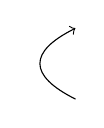
\begin{tikzpicture}[x=3mm,y=3mm]\draw[->] (1,0) .. controls (-1,1) and (-1,2) .. (1,3);\end{tikzpicture}}

\diagram{\deleted{\mbox{\begin{tikzcd}[ampersand replacement=\&,row sep=1ex,column sep=1em,execute at end picture={\draw (current bounding box.south west) rectangle (current bounding box.north east);}]
\unsure{4}\arrow[d,dash] \& \& 1\arrow[d,dash,very thick]\arrow[ddrr,dash,very thick] \& \& \& \text{Leitfaden}\\
\unsure{2} \& \& 2\arrow[d,dash,very thick]\arrow[dl,dash] \& \& \& \\
\& \unsure{5} \& 3\arrow[dr,dash]\arrow[d,dash] \& \deleted{\unsure{2}}\arrow[r,dash] \& 6\arrow[d,dash,thick] \& \\
\& \& \unsure{4} \& 4\arrow[dr,dash] \& \deleted{\unsure{3}} \& \\
\& \& \& \& 7 \&
\end{tikzcd}}}}

\diagram{\begin{tikzcd}[ampersand replacement=\&,row sep=1ex,column sep=1em,execute at end picture={\draw (current bounding box.south west) rectangle (current bounding box.north east);}]
\&1\arrow[d,dash,very thick] \& \& \\
\&2\arrow[d,dash,thick]\arrow[dl,dash]\arrow[ddrr,dash,very thick] \& \& \deleted{\unsure{5|6}}\\
5\&3\arrow[dr,dash]\&\&\\
\&\&4\arrow[dr,dash]\&6\arrow[d,dash,thick]\\
\&\&\&7
\end{tikzcd}}

\margin{\unsure{6.110|6.10}}

% archive sheet number: 32
\scanpage{34}
\deleted{\deleted{\unsure{Soit|Théorème}} Soit $F$ un faisceau de $l$-torsion sur $Y$, et soit $\xi\unsure{\in|\,} H^n(X,f^*(F))$. Pour que $\xi\in\mathrm{Im}\ H^n(Y,F)$, il f. et s. que pour \deleted{tout} $y\in Y$, la classe $\xi_{\bar y}\in H^n(X_{\bar y},F_{\bar y})$ \deleted{\unsure{induit|induite}} sur la fibre géométrique de $X_{\bar y}$ soit nulle.}

\margin{\deleted{\unsure{IX|X}}}

\deleted{\uline{Corollaire} Supposons $f$ \inserted{qu. cp et} localemt $(n,\unsure{\,|\ell})$-acyclique pour $l$. Pour qu'il soit \uline{globalemt} $n$-acyclique pour $l$, il f. et s. que ses fibres géométriques soient $n$-acycliques pour $l$.}

\margin{$Y$ loc. noeth.}

\deleted{Dém. du th. 2.}

\deleted{Par hypothèse on a}
\[
\deleted{\left\{\begin{aligned}
R^q f_*(f^*(F))&=0 &&\text{pour }0<q\le n-1\\
R^{\unsure{0|q}}f_*(f^*(G))&\simeq G
\end{aligned}\right.}
\]

\deleted{donc la \deleted{suite} spectrale donne une suite exacte [NB. on suppose $n-1\ge0$ i.e., $n\ge1$\,; si $n=0$, \unsure{et|est} \unsure{mérite|nécessite} un énoncé séparé avec le \unsure{gpe|prop} fond.]}
\[
\deleted{\unsure{-|\longrightarrow|\cdots\longrightarrow} H^{\unsure{n}}(Y,F)\to H^n(X,F)\to H^0(Y,R^n f_*f^*(F))}
\]

\deleted{donc on est ramené à prouver qu'une section de $R^n f_*(f^*(F))$ qui induit 0 sur chaque fibre géom. est nulle. On est ramené}

% archive sheet number: 33
